%% FEUP THESIS STYLE for LaTeX2e
%% how to use feupteses (English version)
%%
%% FEUP, JCL & JCF, 31 July 2012
%%
%% Read the documentation inline and
%% at https://web.fe.up.pt/~jlopes/doku.php/teach/feupteses
%%
%% PLEASE send improvements to jlopes at fe.up.pt and to jcf at fe.up.pt
%%

%%========================================
%% Commands: pdflatex meic_thesis
%%           bibtex meic_thesis
%%           makeindex meic_thesis (only if creating an index)
%%           pdflatex meic_thesis
%% Alternative:
%%           latexmk -pdf meic_thesis.tex
%% Using the Makefile:
%%           make
%%========================================

%% 2021-07-20: One-sided output by default
\documentclass[11pt,a4paper]{report}

%% For two-sided printing (for dead-tree output) comment previous line
%% and uncomment the next line
%\documentclass[11pt,a4paper,twoside,openright]{report}

%% For iso-8859-1 (latin1), comment next line and uncomment the second line
\usepackage[utf8]{inputenc}
%\usepackage[latin1]{inputenc}

%% English version

%% MEIC options
\usepackage[meic]{feupteses}                  % work version
%\usepackage[meic,juri]{feupteses}             % jury version
%\usepackage[meic,final]{feupteses}            % final version
%\usepackage[meic,final,onpaper]{feupteses}    % final on paper version

%% Additional options for feupteses.sty: 
%% - portugues: titles, etc in portuguese
%% - onpaper: links are not shown (for paper versions)
%% - backrefs: include back references from bibliography to citation place

%% Uncomment the next lines if side by side graphics used
\usepackage[lofdepth,lotdepth]{subfig}
\usepackage{graphicx}
\usepackage{float}

% Listings
\definecolor{cloudwhite}{cmyk}{0,0,0,0.025}  % color

%% Include source-code listings package
\usepackage{listings}
\lstset{ %
 language=C,                        % choose the language of the code
 basicstyle=\footnotesize\ttfamily,
 keywordstyle=\bfseries,
 numbers=left,                      % where to put the line-numbers
 numberstyle=\scriptsize\texttt,    % the size of the fonts that are used for the line-numbers
 stepnumber=1,                      % the step between two line-numbers. If it's 1 each line will be numbered
 numbersep=8pt,                     % how far the line-numbers are from the code
 frame=tb,
 float=htb,
 aboveskip=8mm,
 belowskip=4mm,
 backgroundcolor=\color{cloudwhite},
 showspaces=false,                  % show spaces adding particular underscores
 showstringspaces=false,            % underline spaces within strings
 showtabs=false,                    % show tabs within strings adding particular underscores
 tabsize=2,                         % sets default tabsize to 2 spaces
 captionpos=b,                      % sets the caption-position to bottom
 breaklines=true,                   % sets automatic line breaking
 breakatwhitespace=false,           % sets if automatic breaks should only happen at whitespace
 escapeinside={\%*}{*)},            % if you want to add a comment within your code
 morekeywords={*,var,template,new}  % if you want to add more keywords to the set
}

%%Uncomment to create an index (at the end of the document)
%\makeindex

%% Path to the figures directory
%% TIP: use folder ``figures'' to keep all your figures
\graphicspath{{figures/}}

%%========================================
%% Start of document
%%========================================
\begin{document}

%%----------------------------------------
%% TIP: if you want to define more macros, use an external file to keep them
%% some macro definitions

% format
\newcommand{\class}[1]{{\normalfont\slshape #1\/}}

% entities
\newcommand{\Feup}{Faculdade de Engenharia da Universidade do Porto}

\newcommand{\svg}{\class{SVG}}
\newcommand{\scada}{\class{SCADA}}
\newcommand{\scadadms}{\class{SCADA/DMS}}

%%----------------------------------------

%%----------------------------------------
%% Information about the work
%%----------------------------------------
\title{Title of the Dissertation}
\author{Name of the Author}

%% Comment next line if not necessary for degree
%\degree{Programa Doutoral em Engenharia Informática}

%% Uncomment next line for date of submission
%\thesisdate{July 31, 2008}

%% Comment next line copyright text if not used
%\copyrightnotice{Name of the Author, 2008}

\supervisor{Supervisor}{Prof.\ Name of the Supervisor}

%% Uncomment next line if necessary
%\supervisor{Second Supervisor}{Prof.\Name of the Supervisor}

%% Uncomment committee stuff in the final version
%\committeetext{Approved in oral examination by the committee:}
%\committeemember{President}{Prof.\ Name of the President}
%\committeemember{Referee}{Prof.\ Name of the Referee}
%\committeemember{Referee}{Prof.\ Name of the Referee}

%\committeetext{Aprovado em provas públicas pelo Júri:}
%\committeemember{Presidente}{Prof.\ Nome do presidente do júri}
%\committeemember{Arguente}{Prof.\ Nome do arguente do júri}
%\committeemember{Vogal}{Prof.\ Nome do vogal do júri}

%% Uncomment signature line in the final on paper version if used
%\signature

%% Specify cover logo (in folder ``figures'')
\logo{uporto-feup.pdf}

%% Uncomment next line for additional text below the author's name (front page)
% \additionalfronttext{Preparação da Dissertação}
%\additionalfronttext{Dissertation Planning}

%%----------------------------------------
%% Preliminary materials
%%----------------------------------------

% remove unnecessary \include{} commands
\begin{Prolog}
  \chapter*{Resumo}
%\addcontentsline{toc}{chapter}{Resumo}

Este documento ilustra o formato a usar em dissertações na \Feup.
São dados exemplos de margens, cabeçalhos, títulos, paginação, estilos
de índices, etc. 
São ainda dados exemplos de formatação de citações, figuras e tabelas,
equações, referências cruzadas, lista de referências e índices.
Este documento não pretende exemplificar conteúdos a usar. 
É usado o \emph{Loren Ipsum} para preencher a dissertação.

Lorem ipsum dolor sit amet, consectetuer adipiscing elit. Etiam vitae
quam sed mauris auctor porttitor. Mauris porta sem vitae arcu sagittis
facilisis. Proin sodales risus sit amet arcu. Quisque eu pede eu elit
pulvinar porttitor. Maecenas dignissim tincidunt dui. Pellentesque
habitant morbi tristique senectus et netus et malesuada fames ac
turpis egestas. Donec non augue sit amet nulla gravida
rutrum. Vestibulum ante ipsum primis in faucibus orci luctus et
ultrices posuere cubilia Curae; Nunc at nunc. Etiam egestas. 

Donec malesuada pede eget nunc. Fusce porttitor felis eget mi mattis
vestibulum. Pellentesque faucibus. Cras adipiscing dolor quis
mi. Quisque sagittis, justo sed dapibus pharetra, lectus velit
tincidunt eros, ac fermentum nulla velit vel sapien. Vestibulum sem
mauris, hendrerit non, feugiat ac, varius ornare, lectus. Praesent
urna tellus, euismod in, hendrerit sit amet, pretium vitae,
nisi. Proin nisl sem, ultrices eget, faucibus a, feugiat non,
purus. Etiam mi tortor, convallis quis, pharetra ut, consectetuer eu,
orci. Vivamus aliquet. Aenean mollis fringilla erat. Vivamus mollis,
purus at pellentesque faucibus, sapien lorem eleifend quam, mollis
luctus mi purus in dui. Maecenas volutpat mauris eu lectus. Morbi vel
risus et dolor bibendum malesuada. Donec feugiat tristique erat. Nam
porta auctor mi. Nulla purus. Nam aliquam. 

\chapter*{Abstract}
%\addcontentsline{toc}{chapter}{Abstract}

Here goes the abstract written in English.

Lorem ipsum dolor sit amet, consectetuer adipiscing elit. Sed vehicula
lorem commodo dui. Fusce mollis feugiat elit. Cum sociis natoque
penatibus et magnis dis parturient montes, nascetur ridiculus
mus. Donec eu quam. Aenean consectetuer odio quis nisi. Fusce molestie
metus sed neque. Praesent nulla. Donec quis urna. Pellentesque
hendrerit vulputate nunc. Donec id eros et leo ullamcorper
placerat. Curabitur aliquam tellus et diam. 

Ut tortor. Morbi eget elit. Maecenas nec risus. Sed ultricies. Sed
scelerisque libero faucibus sem. Nullam molestie leo quis
tellus. Donec ipsum. Nulla lobortis purus pharetra turpis. Nulla
laoreet, arcu nec hendrerit vulputate, tortor elit eleifend turpis, et
aliquam leo metus in dolor. Praesent sed nulla. Mauris ac augue. Cras
ac orci. Etiam sed urna eget nulla sodales venenatis. Donec faucibus
ante eget dui. Nam magna. Suspendisse sollicitudin est et mi. 

Fusce sed ipsum vel velit imperdiet dictum. Sed nisi purus, dapibus
ut, iaculis ac, placerat id, purus. Integer aliquet elementum
libero. Phasellus facilisis leo eget elit. Nullam nisi magna, ornare
at, aliquet et, porta id, odio. Sed volutpat tellus consectetuer
ligula. Phasellus turpis augue, malesuada et, placerat fringilla,
ornare nec, eros. Class aptent taciti sociosqu ad litora torquent per
conubia nostra, per inceptos himenaeos. Vivamus ornare quam nec sem
mattis vulputate. Nullam porta, diam nec porta mollis, orci leo
condimentum sapien, quis venenatis mi dolor a metus. Nullam
mollis. Aenean metus massa, pellentesque sit amet, sagittis eget,
tincidunt in, arcu. Vestibulum porta laoreet tortor. Nullam mollis
elit nec justo. In nulla ligula, pellentesque sit amet, consequat sed,
faucibus id, velit. Fusce purus. Quisque sagittis urna at quam. Ut eu
lacus. Maecenas tortor nibh, ultricies nec, vestibulum varius, egestas
id, sapien. 

Donec hendrerit. Vivamus suscipit egestas nibh. In ornare leo ut
massa. Donec nisi nisl, dignissim quis, faucibus a, bibendum ac,
diam. Nam adipiscing hendrerit mi. Morbi ac nulla. Nullam id est ac
nisi consectetuer commodo. Pellentesque aliquam massa sit amet
tellus. Vivamus sodales aliquam leo. 
 % the abstract
  \chapter*{Acknowledgements}
\addcontentsline{toc}{chapter}{Acknowledgements}


I want to express my heartfelt gratitude to everyone who contributed, both directly and indirectly, to the completion of this work.

First and foremost, I am profoundly thankful to the professors who have guided me throughout my academic journey. They have played a crucial role in my intellectual and personal development.
I extend my deep appreciation to the INESC TEC team, and particularly to Eduardo Rodrigues, for their invaluable guidance, collaboration, and unwavering support throughout the course of this research.

Additionally, I acknowledge the presence and contributions of all the students who have passed through this faculty. Their shared experiences fostered a stimulating academic and social environment.
A special note of recognition goes to the Academic Traditions, which I wholeheartedly embraced. These traditions significantly enriched my university experience and deepened my sense of belonging to this academic community.

I am immensely grateful to my girlfriend for her steadfast support, patience, and encouragement during the most challenging moments of my academic journey.
To my friends who stood by me over the past five years, providing companionship, motivation, and balance: thank you. I leave with my heart full of our long conversations, unforgettable memories, and the strength drawn from both the joyful and difficult times we shared together.
Finally, I express my deep appreciation to my family, whose unwavering support has always been my foundation. I am especially grateful to my father, whose words have consistently reminded me of the value of resilience: “A vida é dura para quem é mole”

The fight against cancer, which serves as the primary motivation for this research, arises from many years of personal struggle and progress in my health journey. I am profoundly grateful to have reached a point where I can contribute, albeit in a modest way, to alleviating the hardship faced by families impacted by this disease.

This work would not have been achievable without the unwavering support of numerous individuals. Success is never a solitary endeavour, and this dissertation stands as a testament to that truth.

As the Orfeão Universitário do Porto sings: "Quero ficar sempre estudante"\\
With love,\\
Engineering!

\vspace{10mm}
\flushleft{João Malva}

\chapter*{Institutional Acknowledgements}

This work is co-financed by Component 5 - Capitalization and Business Innovation, integrated in the Resilience Dimension of the Recovery and Resilience Plan within the scope of the Recovery and Resilience Mechanism~(MRR) of the European Union~(EU), framed in the Next Generation EU, for the period 2021 - 2026, within project HfPT, with reference 41.

\vspace{10mm}
\flushleft{João Malva}
  % the acknowledgments
  %% This section is optional and can be removed
\cleardoublepage
\thispagestyle{plain}

\vspace*{8cm}

\begin{flushright}
   \textsl{``On ne voit bien qu’avec le coeur. L’essentiel est invisible pour les yeux.''} \\
\vspace*{1.5cm}
    Antoine de Saint-Exupéry
\end{flushright}
    % initial quotation if desired
  \cleardoublepage
  \pdfbookmark[0]{Table of Contents}{contents}
  \tableofcontents
  \cleardoublepage
  \pdfbookmark[0]{List of Figures}{figures}
  \listoffigures
  \cleardoublepage
  \pdfbookmark[0]{List of Tables}{tables}
  \listoftables
  \cleardoublepage
  \pdfbookmark[0]{List of Listings}{listings}
  \lstlistoflistings
  %\chapter*{List of Acronyms}
%\chaptermark{LIST OF ACRONYMS}
%
%\begin{flushleft}
%\begin{tabular}{l p{0.8\linewidth}}
%ADT      & Abstract Data Type\\
%ANDF     & Architecture-Neutral Distribution Format\\
%API      & Application Programming Interface\\
%CAD      & Computer-Aided Design\\
%CASE     & Computer-Aided Software Engineering\\
%CORBA    & Common Object Request Broker Architecture\\
%UNCOL    & UNiversal COmpiler-oriented Language\\
%Loren    & Lorem ipsum dolor sit amet, consectetuer adipiscing
%elit. Sed vehicula lorem commodo dui\\
%WWW      & \emph{World Wide Web}
%\end{tabular}
%\end{flushleft}
%
\chapter*{Abbreviations}
%\addcontentsline{toc}{chapter}{Abbreviations}
\chaptermark{Abbreviations}

\begin{flushleft}

\begin{acronym}[Abbreviations]
    \acro{acrin}[ACRIN]{American College of Radiology Imaging Network}
    \acro{agv}[AGV]{Absolute Gradient Value}
    \acro{agm}[AGM]{Absolute Gradient Matrix}
    \acro{ai}[AI]{Artificial Intelligence}
    \acro{aln}[ALN]{Axillary Lymph Node}
    \acro{anode09}[ANODE09]{Automatic Nodule Detection 2009}
    \acro{asm}[ASM]{Angular Second Momentum}
    \acro{auc}[AUC]{Area Under the Curve}
    \acro{auc-roc}[AUC-ROC]{Area Under the ROC}
    \acro{avg-predict}[AVG-Predict]{Average Prediction Score}
    \acro{bb}[BB]{Bounding Box}
    \acro{bpnn}[BPNN]{Back Propagation Neural Network}
    \acro{cad}[CAD]{Computer-Aided Diagnosis}
    \acro{cam}[CAM]{Class Activation Mapping}
    \acro{cbam}[CBAM]{Convolutional Block Attention Module}
    \acro{cca}[CCA]{Canonical Correlation Analysis}
    \acro{cnn}[CNN]{Convolutional Neural Network}
    \acro{ct}[CT]{Computed Tomography}
    \acro{dce-mri}[DCE-MRI]{Dynamic Contrast-Enhanced \ac{mri}}
    \acro{dcnn}[DCNN]{Deep Convolutional Neural Network}
    \acro{dl}[DL]{Deep Learning}
    \acro{dnn}[DNN]{Deep Neural Network}
    \acro{el}[EL]{Energy Layer}
    \acro{fda}[FDA]{Food and Drug Administration}
    \acro{flops}[FLOPS]{Floating Point Operations per Second}
    \acro{fn}[FN]{False Negative}
    \acro{fnih}[FNIH]{Foundation for the National Institutes of Health}
    \acro{fof}[FOF]{First-Order Features}
    \acro{fp}[FP]{False Positive}
    \acro{fc}[FC]{Fully Connected}
    \acro{gcn}[GCN]{Graph Convolutional Network}
    \acro{gelu}[GELU]{Gaussian Error Linear Unit}
    \acro{glcm}[GLCM]{Gray-Level Co-Occurrence Matrix}
    \acro{glpp}[GLPP]{Global-Local Pyramid Pattern}
    \acro{gpu}[GPU]{Graphics Processing Unit}
    \acro{gtsdm}[GTSDM]{Gray-Tone Spatial Dependence Matrix}
    \acro{hog}[HOG]{Histogram of Oriented Gradients}
    \acro{hu}[HU]{Hounsfield Units}
    \acro{idm}[IDM]{Inverse Difference Momentum}
    \acro{imc}[IMC]{Information Measures of Correlation}
    \acro{iqr}[IQR]{Interquartile Range}
    \acro{knn}[KNN]{K-Nearest Neighbor}
    \acro{lbp}[LBP]{Local Binary Patterns}
    \acro{lidc-idri}[LIDC-IDRI]{Lung Image Database Consortium Image Collection}
    \acro{lnva}[LNVA]{Lung Nodule Visual Attribute}
    \acro{lnm}[LNM]{Lung Nodule Malignancy}
    \acro{lss}[LSS]{Lung Screening Study group}
    \acro{lstm}[LSTM]{Long Short-Term Memory}
    \acro{ltp}[LTP]{Local Trinary Pattern}
    \acro{luna16}[LUNA16]{Lung Nodule Analysis 2016}
    \acro{mad}[MAD]{Mean Absolute Deviation}
    \acro{max-vote}[MAX-VOTE]{Majority Voting}
    \acro{mcc}[MCC]{Maximal Correlation Coefficient}
    \acro{ml}[ML]{Machine Learning}
    \acro{mri}[MRI]{Magnetic Resonance Imaging}
    \acro{nci}[NCI]{National Cancer Institute}
    \acro{nelson}[NELSON]{Nederlands–Leuvens Longkanker Screenings Onderzoek}
    \acro{nlst}[NLST]{National Lung Screening Trial}
    \acro{pca}[PCA]{Principal Component Analysis}
    \acro{pet}[PET]{Positron Emission Tomography}
    \acro{relu}[ReLU]{Rectified Linear Unit}
    \acro{resnet}[ResNet]{Residual Network}
    \acro{rmad}[rMAD]{Robust Mean Absolute Deviation}
    \acro{rms}[RMS]{Root Mean Squared}
    \acro{roi}[ROI]{Region of Interest}
    \acro{sdg}[SDG]{Sustainable Development Goal}
    \acro{shap}[SHAP]{SHapley Additive exPlanations}
    \acro{svm}[SVM]{Support Vector Machine}
    \acro{svm-ffcat}[SVM-FFCAT]{SVM - Feature Fusion by Concatenation}
    \acro{tcia}[TCIA]{The Cancer Imaging Archive}
    \acro{t-lstm}[T-LSTM]{Time-Modulated Long Short-Term Memory}
    \acro{tnm}[TNM]{Tumor-Nodules-Metastasis}
    \acro{tn}[TN]{True Negative}
    \acro{tp}[TP]{True Positive}
    \acro{xai}[XAI]{Explainable Artificial Intelligence}
    
    %\newacronym
    %\newacronym{acc}{ACC}{Accuracy}
\end{acronym}

\end{flushleft}  % the list of abbreviations used
\end{Prolog}

%%----------------------------------------
%% Body
%%----------------------------------------
\StartBody

%% TIP: use a separate file for each chapter
\chapter{Introduction} \label{chap:intro}

This document illustrates the format to be used for dissertations at FEUP.
Examples of margins are given, headings, titles, pagination, index styles, 
etc. are given. 
It also gives examples of formatting citations, figures and tables, 
equations, cross-references, reference lists and indexes. 
This document is not intended to exemplify content to be used.

A collection of existing standards can be found in~\textcite{kn:Mat93}.

This first chapter illustrates the use of citations and references.

\section{Section Example} \label{sec:se1}

As well as giving an example of how to use a quotation, the 
following paragraph introduces a reference that can be consulted, 
among many other interesting bibliographical 
references~\parencite{kn:Tha01,kn:PP05}.

\begin{quote}
  ``Like the Abstract, the Introduction should be written to engage the
  interest of the reader. It should also give the reader an idea of
  how the dissertation is structured, and in doing so, define the
  thread of the contents.''~\parencite[chap.\ Introduction]{kn:Tha01} 
\end{quote}

Lorem ipsum~\textcite{kn:Lip08} dolor sit amet, consectetuer adipiscing
elit. 
Sed eget nunc. Phasellus interdum, risus viverra mollis laoreet, felis
justo iaculis ante, eget ornare purus augue non urna. Nam in magna. 
In a est. Phasellus a tellus vitae enim vehicula imperdiet. 
Etiam sit amet elit. In hac habitasse platea dictumst. 
Quisque eget turpis vel felis elementum tempus. Curabitur sit 
amet tortor id libero dapibus pretium. 
Integer mattis eros eu lorem. Duis erat tellus, porttitor
sed, blandit eget, fringilla et, lacus. Phasellus tristique nibh nec
orci. Mauris sed leo. Suspendisse fringilla tempor dolor. Donec sapien
enim, congue in, porta et, sollicitudin in, quam. Curabitur semper,
mauris ut vestibulum eleifend, diam ipsum tincidunt quam, et
vestibulum velit mauris ut risus. 

Sed eget libero. Nulla facilisi. Proin eget tortor. Morbi
gravida. Donec arcu risus, blandit a, rutrum at, ornare ut,
nisl. Etiam consectetuer tortor eu odio. Etiam blandit molestie
ligula. Nulla facilisi. Nam a augue non justo laoreet hendrerit. Nam
aliquam, purus eu ultricies dictum, urna purus posuere neque, vel
tempus tellus enim a arcu. 

Pellentesque congue sapien in ligula. Nulla nec mi sed augue congue
tristique. Cras pretium. Pellentesque lobortis, libero id adipiscing
auctor, orci massa vehicula nulla, vel ullamcorper tortor ipsum ut
elit. Morbi rhoncus, dui sed tristique volutpat, lorem felis euismod
lorem, vel tristique nibh arcu vel eros. Nunc tempor. Sed et erat a
tortor fermentum consequat. Cras varius nisl accumsan libero. Aliquam
faucibus, justo ut pharetra blandit, est nibh ultrices est, vel
facilisis quam lectus ut enim. Aliquam convallis, nibh non bibendum
pharetra, nisl velit lobortis orci, ac ultrices neque sem viverra
massa. Donec malesuada. Aliquam ligula. Fusce in nisl. Etiam lacinia
est quis velit. Maecenas massa. Maecenas sed pede. Nulla
sodales. Etiam vitae erat. Duis tristique sem sit amet libero. Ut a
libero nec ligula tempus mattis. 

\section{Section Example} \label{sec:ae2}

Lorem ipsum dolor sit amet, consectetuer adipiscing elit. Morbi sit
amet nibh. Fusce faucibus, enim vel ultrices ornare, est mauris
ultricies velit, vitae consequat sem erat vel nunc. Nam libero eros,
mattis eget, sagittis nec, imperdiet at, sapien. Aliquam lacus. Aenean
adipiscing nibh in orci. Aliquam vestibulum, elit at fringilla
dignissim, metus diam lobortis urna, a laoreet nunc odio ac ipsum. Sed
at urna. Integer vehicula fringilla augue. Nulla lacus eros, rhoncus
sit amet, posuere ut, vehicula ac, nibh. Ut eleifend, eros eu placerat
vehicula, justo turpis blandit dolor, eu tincidunt felis risus at
ante. Aenean suscipit nisl eget eros. Ut laoreet libero eget
enim. Cras tempus pellentesque felis. Vestibulum vitae erat ac nibh
posuere eleifend. 

Integer nec quam. Sed fermentum. Nunc vitae leo. Etiam sit amet
quam. Nunc vestibulum massa in mauris. Duis eget nulla. Fusce
ultricies arcu eu nibh volutpat feugiat. Maecenas urna pede, commodo
quis, porta eu, bibendum elementum, pede. Sed eros massa, molestie
eget, mattis non, rutrum ac, magna. Duis dui. Maecenas eget tortor ut
dolor semper mattis. Maecenas auctor, tellus et ultricies tempor, elit
est placerat lacus, in posuere mauris lorem et arcu. 

Nulla nec eros et pede vehicula aliquam. Aenean sodales pede vel
ante. Fusce sollicitudin sodales lacus. Maecenas justo mauris,
adipiscing vitae, ornare quis, convallis nec, eros. Etiam laoreet
venenatis ipsum. In tellus odio, eleifend ac, ultrices vel, lobortis
sed, nibh. Fusce nunc augue, dictum non, pulvinar sed, consectetuer
eu, ipsum. Vivamus nec pede. Pellentesque pulvinar fringilla dolor. In
sit amet pede. Proin orci justo, semper vel, vulputate quis, convallis
ac, nulla. Nulla at justo. Mauris feugiat dolor. Etiam posuere
fermentum eros. Morbi nisl ipsum, tempus id, ornare quis, mattis id,
dolor. Aenean molestie metus suscipit dolor. Aliquam id lectus sed
nisl lobortis rhoncus. Curabitur vitae diam sed sem aliquet
tempus. Sed scelerisque nisi nec sem. 

\section{Section Example} \label{sec:ae3}

Integer nec quam. Sed fermentum. Nunc vitae leo. Etiam sit amet
quam. Nunc vestibulum massa in mauris. Duis eget nulla. Fusce
ultricies arcu eu nibh volutpat feugiat. Maecenas urna pede, commodo
quis, porta eu, bibendum elementum, pede. Sed eros massa, molestie
eget, mattis non, rutrum ac, magna. Duis dui. Maecenas eget tortor ut
dolor semper mattis. Maecenas auctor, tellus et ultricies tempor, elit
est placerat lacus, in posuere mauris lorem et arcu. 

Nulla nec eros et pede vehicula aliquam. Aenean sodales pede vel
ante. Fusce sollicitudin sodales lacus. Maecenas justo mauris,
adipiscing vitae, ornare quis, convallis nec, eros. Etiam laoreet
venenatis ipsum. In tellus odio, eleifend ac, ultrices vel, lobortis
sed, nibh. Fusce nunc augue, dictum non, pulvinar sed, consectetuer
eu, ipsum. Vivamus nec pede. Pellentesque pulvinar fringilla dolor. In
sit amet pede. Proin orci justo, semper vel, vulputate quis, convallis
ac, nulla. Nulla at justo. Mauris feugiat dolor. Etiam posuere
fermentum eros. Morbi nisl ipsum, tempus id, ornare quis, mattis id,
dolor. Aenean molestie metus suscipit dolor. Aliquam id lectus sed
nisl lobortis rhoncus. Curabitur vitae diam sed sem aliquet
tempus. Sed scelerisque nisi nec sem. 

\section{Section Example} \label{sec:ae4}

Integer nec quam. Sed fermentum. Nunc vitae leo. Etiam sit amet
quam. Nunc vestibulum massa in mauris. Duis eget nulla. Fusce
ultricies arcu eu nibh volutpat feugiat. Maecenas urna pede, commodo
quis, porta eu, bibendum elementum, pede. Sed eros massa, molestie
eget, mattis non, rutrum ac, magna. Duis dui. Maecenas eget tortor ut
dolor semper mattis. Maecenas auctor, tellus et ultricies tempor, elit
est placerat lacus, in posuere mauris lorem et arcu. 

Nulla nec eros et pede vehicula aliquam. Aenean sodales pede vel
ante. Fusce sollicitudin sodales lacus. Maecenas justo mauris,
adipiscing vitae, ornare quis, convallis nec, eros. Etiam laoreet
venenatis ipsum. In tellus odio, eleifend ac, ultrices vel, lobortis
sed, nibh. Fusce nunc augue, dictum non, pulvinar sed, consectetuer
eu, ipsum. Vivamus nec pede. Pellentesque pulvinar fringilla dolor. In
sit amet pede. Proin orci justo, semper vel, vulputate quis, convallis
ac, nulla. Nulla at justo. Mauris feugiat dolor. Etiam posuere
fermentum eros. Morbi nisl ipsum, tempus id, ornare quis, mattis id,
dolor. Aenean molestie metus suscipit dolor. Aliquam id lectus sed
nisl lobortis rhoncus. Curabitur vitae diam sed sem aliquet
tempus. Sed scelerisque nisi nec sem. 

\section{Dissertation Structure} \label{sec:struct}

In addition to the introduction, this dissertation contains x more 
chapters.

In Chapter~\ref{chap:ch2}, the state of the art is described and 
related work is presented. 
Chapter~\ref{chap:ch3}, ipsum dolor sit amet, consectetuer
adipiscing elit.
 
\chapter{Chapter Example} \label{chap:ch2}

Lorem ipsum dolor sit amet, consectetuer adipiscing elit. Donec a
eros. Phasellus non nulla non massa venenatis convallis. In
porta. Mauris quis magna. 

\section{Introduction}

Fusce risus mi, tristique eu, consectetuer id, auctor sed, elit. Donec
laoreet. Duis consectetuer interdum libero~\textcite{kn:MVL06-xata}.

In euarcu. Fusce luctus diam eget lectus. Duis interdum lacus sed
ligula. Proin vestibulum felis eget lacus. Vivamus vestibulum, tellus
ut congue viverra, mauris lacus tempor turpis, eu congue nisi magna at
dolor. Ut molestie vehicula libero. Praesent in neque sed risus tempus
ornare. Donec hendrerit, erat eu semper aliquam, pede nulla dapibus
risus, ut pretium orci pede et neque.
Etiam eget tortor a metus convallis viverra. Quisque eget nisi sed
orci facilisis interdum. Aliquam non felis. 

\section{Section Example}\label{sec:se21}

\emph{Scalable Vector Graphics}\index{SVG}\index{XML!SVG} 
Curabitur ipsum tortor, ornare vitae, dapibus pretium, 
hendrerit sed, urna.~\parencite{kn:svgdoc}.

Lorem ipsum dolor sit amet, consectetuer adipiscing elit. Donec a
eros. Phasellus non nulla non massa venenatis convallis. In
porta. Mauris quis magna.~\textcite{kn:svgibm,kn:svgw3c}.

Lorem ipsum dolor sit amet, consectetuer adipiscing elit. Donec a
eros. Phasellus non nulla non massa venenatis convallis. In
porta. Mauris quis magna. Proin mauris eros, aliquet id, eleifend
vitae, semper quis, erat. Aliquam id lectus non odio dignissim
blandit. Vestibulum porttitor arcu ut ligula.

Vestibulum ante ipsum primis in faucibus orci luctus et
ultrices posuere cubilia Curae; Phasellus bibendum, nulla eget varius
aliquam, tortor nulla sollicitudin quam, vel vestibulum nisl magna at
sem. Aliquam velit sapien, ultrices viverra, tempus quis, ultrices at,
dui. Aliquam sit amet justo. Quisque tristique, metus eu iaculis
sagittis, urna leo bibendum diam, a ultricies sem diam a augue. Mauris
consectetuer, libero vel euismod tincidunt, nisi metus viverra ante,
quis pretium sapien odio nec risus. Nunc semper auctor
nulla\footnote{Example of a footnote.}. 

\subsection{Subsection Example} \label{sec:se311}

Lorem ipsum dolor sit amet, consectetuer adipiscing elit. Nunc eu
nulla. Pellentesque vitae nibh ultrices quam iaculis
convallis. Aliquam purus eros, varius eget, volutpat sodales,
imperdiet nec, lacus \textit{applets}~\parencite{kn:batik}. 

Curabitur in elit sed sem rutrum posuere. Class aptent taciti 
sociosqu ad litora torquent per conubia nostra, per
inceptos himenaeos~\parencite{kn:svgdoc}. 

Lorem ipsum dolor sit amet, consectetuer adipiscing elit. Nunc eu
nulla. Pellentesque vitae nibh ultrices quam iaculis
convallis. Aliquam purus eros, varius eget, volutpat sodales,
imperdiet nec, lacus. Curabitur in elit sed sem rutrum posuere. Class
aptent taciti sociosqu ad litora torquent per conubia nostra, per
inceptos himenaeos. Duis sem. Praesent ultricies odio vel
sapien. Integer faucibus malesuada libero. Cras semper, dolor id
ullamcorper varius, magna risus volutpat felis, id pellentesque nulla
ante at erat. Integer sodales. 

Quisque sit amet odio. In at risus sit amet turpis interdum
posuere. Maecenas iaculis vehicula sem. Ut leo arcu, malesuada vel,
imperdiet id, dignissim a, purus. Duis eleifend, lectus non venenatis
dignissim, risus libero imperdiet mi, nec gravida massa libero sed
mauris. Nullam lobortis libero non sapien. Integer convallis iaculis
erat. Morbi dictum. Ut ultrices pellentesque velit. Cras ac
ante. Etiam in neque tincidunt lacus gravida vehicula. Proin et nisi. 

Vivamus non nunc nec risus tempor varius. Quisque bibendum mi at
dolor. Aliquam consectetuer condimentum risus. Aliquam luctus pulvinar
sem. Duis aliquam, urna et vulputate tristique, dui elit aliquet nibh,
vel dignissim magna turpis id sapien. Duis commodo sem id
quam. Phasellus dolor. Class aptent taciti sociosqu ad litora torquent
per conubia nostra, per inceptos himenaeos. 

\subsection{Subsection Example} \label{sec:se312}

Loren ipsum dolor sit amet, consectetuer adipiscing elit. 
Praesent sit amet sem. Maecenas eleifend facilisis leo. Vestibulum et
mi. Aliquam posuere, ante non tristique consectetuer, dui elit
scelerisque augue, eu vehicula nibh nisi ac est. Suspendisse elementum
sodales felis. Nullam laoreet fermentum urna. 

Duis eget diam. In est justo, tristique in, lacinia vel, feugiat eget,
quam. Pellentesque habitant morbi tristique senectus et netus et
malesuada fames ac turpis egestas. Fusce feugiat, elit ac placerat
fermentum, augue nisl ultricies eros, id fringilla enim sapien eu
felis. Vestibulum ante ipsum primis in faucibus orci luctus et
ultrices posuere cubilia Curae; Sed dolor mi, porttitor quis,
condimentum sed, luctus in. 

\section{Summary}

Aliquam erat volutpat. Nunc pede ipsum, porttitor eu, bibendum non,
bibendum nec, nisl. Maecenas eget mauris. Nullam pulvinar. Curabitur
rutrum commodo est. Nam sapien pede, interdum eu, accumsan ultrices,
venenatis sit amet, tellus. Praesent ac ante bibendum enim varius
suscipit. Donec enim. Proin nisi. Quisque libero turpis, varius ut,
elementum vel, pulvinar sed, nunc. 

\chapter{Chapter Example} \label{chap:ch3}

Maecenas eleifend facilisis leo. Vestibulum et
mi. Aliquam posuere, ante non tristique consectetuer, dui elit
scelerisque augue, eu vehicula nibh nisi ac est. 
Suspendisse elementum sodales felis. Nullam laoreet fermentum urna. 

\section{Introduction}

Pellentesque rutrum, sapien at viverra 
facilisis\footnote{\url{https://en.wikipedia.org/wiki/Equation}}\footnote{\url{https://www.overleaf.com/learn/latex/Mathematical_expressions}}:

\begin{eqnarray}
CIF_1: \hspace*{5mm}F_0^j(a) &=& \frac{1}{2\pi \iota} \oint_{\gamma} \frac{F_0^j(z)}{z - a} dz\\
CIF_2: \hspace*{5mm}F_1^j(a) &=& \frac{1}{2\pi \iota} \oint_{\gamma} \frac{F_0^j(x)}{x - a} dx \label{eq:cif}
\end{eqnarray}

Equação~\ref{eq:cif} lorem ipsum dolor sit amet, consectetuer
adipiscing elit. Suspendisse tincidunt viverra elit. Donec tempus
vulputate mauris. Donec arcu. Vestibulum condimentum porta
justo. Curabitur ornare tincidunt lacus. Curabitur ac massa vel ante
tincidunt placerat. Cras vehicula semper elit. Curabitur gravida, est
a elementum suscipit, est eros ullamcorper quam, sed cursus velit
velit tempor neque. Duis tempor condimentum ante. Nam
sollicitudin. Vestibulum adipiscing, orci eu tempor dapibus, risus
sapien porta metus, et cursus leo metus eget nibh. 

Pellentesque rutrum, sapien at viverra facilisis, metus eros blandit
sem, quis dictum erat metus eget erat. Vivamus malesuada dapibus
nulla. Maecenas nec purus. Suspendisse auctor mattis augue. Phasellus
enim nisi, iaculis sit amet, pellentesque a, iaculis in, dui. Integer
risus. 

Curabitur ac massa vel ante tincidunt placerat. 
Curabitur gravida, est cras vehicula semper elit
a elementum suscipit, est eros ullamcorper quam, sed cursus velit
velit tempor neque. Duis tempor condimentum ante. Nam
sollicitudin. Vestibulum adipiscing, orci eu tempor dapibus, risus
sapien porta metus, et cursus leo metus eget nibh.

\section{Section Example} \label{sec:se32}

Curabitur ac massa vel ante tincidunt placerat\parencite{kn:ZPMD97}: 

\begin{itemize}
\item \textbf{Components} --- Suspendisse auctor mattis augue \emph{push};
\item \textbf{Praesent} --- Sit amet sem maecenas eleifend facilisis leo;
\item \textbf{Pellentesque} --- Habitant morbi tristique senectus et netus.
\end{itemize}

\subsection{Subsection Example} \label{sec:se321}

Suspendisse elementum sodales felis in Figure~\ref{fig:arch} on 
page~\pageref{fig:arch} is a floating figure.

\begin{figure}
    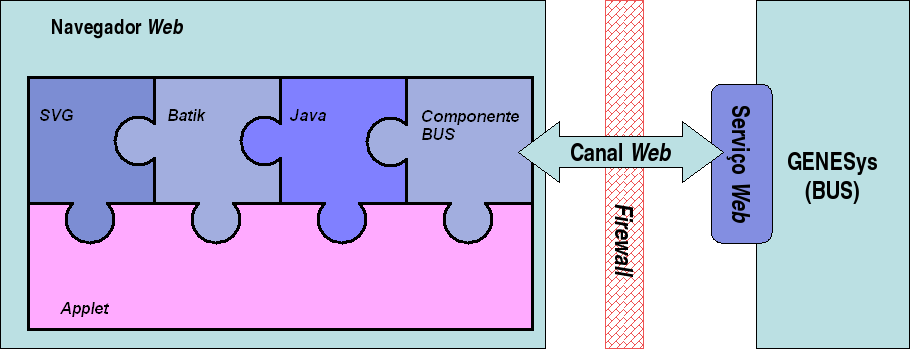
\includegraphics[width=0.86\textwidth]{puzzle}
    \caption{Architecture}
    \label{fig:arch}
\end{figure}

Loren ipsum dolor sit amet, consectetuer adipiscing elit. 
Praesent sit amet sem. Maecenas eleifend facilisis leo. Vestibulum et
mi. Aliquam posuere, ante non tristique consectetuer, dui elit
scelerisque augue, eu vehicula nibh nisi ac est. Nullam laoreet fermentum urna.

Duis eget diam. In est justo, tristique in, lacinia vel, feugiat eget,
quam. Pellentesque habitant morbi tristique senectus et netus et
malesuada fames ac turpis egestas. Fusce feugiat, elit ac placerat
fermentum, augue nisl ultricies eros, id fringilla enim sapien eu
felis. Vestibulum ante ipsum primis in faucibus orci luctus et
ultrices posuere cubilia Curae; Sed dolor mi, porttitor quis,
condimentum sed, luctus in. 

\subsection{Subsection Example} \label{sec:se322}

Suspendisse elementum sodales felis in Table~\ref{tab:example} is a 
floating table.

\begin{table}
  \caption{A table}
\begin{tabular}{|c|r@{.}lr@{.}lr@{.}l||r|}
	\hline
\multicolumn{8}{|c|}
	{\rule[-3mm]{0mm}{8mm}Iteration $k$ de $f(x_n)$} \\
\textbf{\em k}
	& \multicolumn{2}{c}{$x_1^k$}
	& \multicolumn{2}{c}{$x_2^k$}
	& \multicolumn{2}{c||}{$x_3^k$}
	& comments \\ \hline \hline
0   & -0&3                 & 0&6                 &  0&7   & - \\
1   &  0&47102965 & 0&04883157 & -0&53345964  & $\delta<\epsilon$ \\
2   &  0&49988691 & 0&00228830 & -0&52246185  & $\delta < \varepsilon$ \\
3   &  0&49999976 & 0&00005380 & -0&523656   &   $N$ \\
4   &  0&5                 & 0&00000307 & -0&52359743  & \\
\vdots	& \multicolumn{2}{c}{\vdots}
	& \multicolumn{2}{c}{$\ddots$}
	& \multicolumn{2}{c||}{\vdots}  & \\
7   &  0&5   & 0&0    & \textbf{-0}&\textbf{52359878}
		 & $\delta<10^{-8}$ \\ \hline
\end{tabular}
  \label{tab:example}
\end{table}

Loren ipsum dolor sit amet, consectetuer adipiscing elit. 
Praesent sit amet sem. Maecenas eleifend facilisis leo. Vestibulum et
mi. Aliquam posuere, ante non tristique consectetuer, dui elit
scelerisque augue, eu vehicula nibh nisi ac est. Suspendisse elementum
sodales felis. Nullam laoreet fermentum urna. 

Duis eget diam. In est justo, tristique in, lacinia vel, feugiat eget,
quam. Pellentesque habitant morbi tristique senectus et netus et
malesuada fames ac turpis egestas. Fusce feugiat, elit ac placerat
fermentum, augue nisl ultricies eros, id fringilla enim sapien eu
felis. Vestibulum ante ipsum primis in faucibus orci luctus et
ultrices posuere cubilia Curae; Sed dolor mi, porttitor quis,
condimentum sed, luctus in. 

\section{Section Example}

Loren ipsum dolor sit amet, consectetuer adipiscing elit. 
Praesent sit amet sem. Maecenas eleifend facilisis leo. Vestibulum et
mi. Aliquam posuere, ante non tristique consectetuer, dui elit
scelerisque augue, eu vehicula nibh nisi ac est. Suspendisse elementum
sodales felis. Nullam laoreet fermentum urna. 

\section{Summary}

Pellentesque habitant morbi tristique senectus et netus et
malesuada fames ac turpis egestas. Fusce feugiat, elit ac placerat
fermentum, augue nisl ultricies eros, id fringilla enim sapien eu
felis. Vestibulum ante ipsum primis in faucibus orci luctus et
ultrices posuere cubilia Curae; Sed dolor mi, porttitor quis,
condimentum sed, luctus in. 

%%%% Another chapter to force two pages in the index
%%%%
\chapter{Another chapter}

Integer nec quam. Sed fermentum. Nunc vitae leo. Etiam sit amet
quam. Nunc vestibulum massa in mauris. Duis eget nulla. 

\section{Section Example}

Fusce ultricies arcu eu nibh volutpat feugiat. Maecenas urna pede, 
commodo quis, porta eu, bibendum elementum, pede. 

\section{Section Example}

Sed eros massa, molestie eget, mattis non, rutrum ac, magna. 
Duis dui. Maecenas eget tortor ut dolor semper mattis. 
Maecenas auctor, tellus et ultricies tempor, elit
est placerat lacus, in posuere mauris lorem et arcu. 

\subsection{Subsection Example}

Nulla nec eros et pede vehicula aliquam. Aenean sodales pede vel
ante. Fusce sollicitudin sodales lacus. Maecenas justo mauris,
adipiscing vitae, ornare quis, convallis nec, eros. 

\subsection{Subsection Example}

Pellentesque pulvinar fringilla dolor. In sit amet pede. 
Proin orci justo, semper vel, vulputate quis, convallis
ac, nulla. Nulla at justo. Mauris feugiat dolor. 
Etiam posuere fermentum eros. Morbi nisl ipsum, tempus id, 
ornare quis, mattis id, dolor. Aenean molestie metus 
suscipit dolor. Aliquam id lectus sed
nisl lobortis rhoncus. Curabitur vitae diam sed sem aliquet
tempus. Sed scelerisque nisi nec sem.

\section{Section Example}

Sed eros massa, molestie eget, mattis non, rutrum ac, magna. 
Duis dui. Maecenas eget tortor ut dolor semper mattis. 
Maecenas auctor, tellus et ultricies tempor, elit
est placerat lacus, in posuere mauris lorem et arcu. 

\subsection{Subsection Example}

Nulla nec eros et pede vehicula aliquam. Aenean sodales pede vel
ante. Fusce sollicitudin sodales lacus. Maecenas justo mauris,
adipiscing vitae, ornare quis, convallis nec, eros. 

\subsection{Subsection Example}

Aliquam id lectus sed nisl lobortis rhoncus. 
Curabitur vitae diam sed sem aliquet tempus. Sed scelerisque 
nisi nec sem \textcite{khakipoor_linear_2023,liu_energy_2023}.

\section{Section Example}

Maecenas urna pede, commodo quis, porta eu, bibendum elementum, 
pede. Sed eros massa, molestie eget, mattis non, rutrum ac, 
magna. Duis dui. Maecenas eget tortor ut dolor semper mattis. 
Maecenas auctor, tellus et ultricies tempor, elit est placerat 
lacus, in posuere mauris lorem et arcu~\parencite{monopoli_exploiting_2023,zhang_carma_2023,chang_adas_2023, guo_rapidstream_2023}. 

\subsection{Subsection Example}

Nulla nec eros et pede vehicula aliquam. Aenean sodales pede vel
ante. Fusce sollicitudin sodales lacus. Maecenas justo mauris,
adipiscing vitae, ornare quis, convallis nec, eros. 

\subsection{Subsection Example}

Aliquam id lectus sed nisl lobortis rhoncus. 
Curabitur vitae diam sed sem aliquet tempus. Sed scelerisque 
nisi nec sem \textcite{khakipoor_linear_2023,liu_energy_2023} scelerisque.

Nulla nec eros et pede vehicula aliquam. Aenean sodales pede vel
ante. Fusce sollicitudin sodales lacus. Maecenas justo mauris,
adipiscing vitae, ornare quis, convallis nec, eros. Etiam laoreet
venenatis ipsum. In tellus odio, eleifend ac, ultrices vel, lobortis
sed, nibh. Fusce nunc augue, dictum non, pulvinar sed, consectetuer
eu, ipsum. Vivamus nec pede.  

\include{chapter4}
\include{chapter5} 

%%----------------------------------------
%% Final materials
%%----------------------------------------

%% Bibliography
%% Comment the next command if BibTeX file not used
%% bibliography is in ``myrefs.bib''
\PrintBib{myrefs}

%% 2021-07-20: change
%% comment next 2 commands if numbered appendices are not used
\appendix
%% an example of appendix
\chapter{Lorem Ipsum} \label{ap1:Lorem}

After the conclusions and bibliographical references,
the text used to complete the dissertation is presented in this 
numbered annex. 

\section{What is \emph{Lorem Ipsum}?}

\emph{\textbf{Lorem Ipsum}} is simply dummy text of the printing and
typesetting industry. Lorem Ipsum has been the industry's standard
dummy text ever since the 1500s, when an unknown printer took a galley
of type and scrambled it to make a type specimen book. It has survived
not only five centuries, but also the leap into electronic
typesetting, remaining essentially unchanged. It was popularised in
the 1960s with the release of Letraset sheets containing Lorem Ipsum
passages, and more recently with desktop publishing software like
Aldus PageMaker including versions of Lorem Ipsum~\cite{kn:Lip08}. 

\section{Where does \emph{Lorem} come from?}

Contrary to popular belief, Lorem Ipsum is not simply random text. It
has roots in a piece of classical Latin literature from 45 BC, making
it over 2000 years old. Richard McClintock, a Latin professor at
Hampden-Sydney College in Virginia, looked up one of the more obscure
Latin words, consectetur, from a Lorem Ipsum passage, and going
through the cites of the word in classical literature, discovered the
undoubtable source. Lorem Ipsum comes from sections 1.10.32 and
1.10.33 of ``de Finibus Bonorum et Malorum'' (The Extremes of Good and
Evil) by Cicero, written in 45 BC. This book is a treatise on the
theory of ethics, very popular during the Renaissance. The first line
of Lorem Ipsum, ``Lorem ipsum dolor sit amet\ldots'', comes from a line in
section 1.10.32.

The standard chunk of Lorem Ipsum used since the 1500s is reproduced
below for those interested. Sections 1.10.32 and 1.10.33 from ``de
Finibus Bonorum et Malorum'' by Cicero are also reproduced in their
exact original form, accompanied by English versions from the 1914
translation by H. Rackham.

\section{Why is \emph{Lorem} used?}

It is a long established fact that a reader will be distracted by the
readable content of a page when looking at its layout. The point of
using Lorem Ipsum is that it has a more-or-less normal distribution of
letters, as opposed to using ``Content here, content here'', making it
look like readable English. Many desktop publishing packages and web
page editors now use Lorem Ipsum as their default model text, and a
search for ``lorem ipsum'' will uncover many web sites still in their
infancy. Various versions have evolved over the years, sometimes by
accident, sometimes on purpose (injected humour and the like). 

\section{Where can you find examples?}

There are many variations of passages of Lorem Ipsum available, but
the majority have suffered alteration in some form, by injected
humour, or randomised words which don't look even slightly
believable. If you are going to use a passage of Lorem Ipsum, you need
to be sure there isn't anything embarrassing hidden in the middle of
text. All the Lorem Ipsum generators on the Internet tend to repeat
predefined chunks as necessary, making this the first true generator
on the Internet. It uses a dictionary of over 200 Latin words,
combined with a handful of model sentence structures, to generate
Lorem Ipsum which looks reasonable. The generated Lorem Ipsum is
therefore always free from repetition, injected humour, or
non-characteristic words etc. 


%% Index
%% Uncomment next command if index is required
%% don't forget to run ``makeindex thesis'' command
%\PrintIndex

\end{document}
